\documentclass[conference]{IEEEtran}

\usepackage{cite}
\usepackage{amsmath,amssymb,amsfonts}
\usepackage{algorithmic}
\usepackage{graphicx}
\usepackage{textcomp}
\usepackage{xcolor}
\usepackage{amsmath}
\usepackage{hyperref}
\newcommand{\vers}[1]{\hat{\textbf{#1}}}
\newcommand{\vect}[1]{\textbf{#1}}
\newcommand{\norm}[1]{\left\lVert #1\right\rVert}

\begin{document}

\title{Active Contraints in robot-assisted minimally invasive surgery}

\author{ Nicolò Pasini\\
\textit{Person Code: 10576999 } \\
\textit{Student Number: 971406}\\
\href{mailto:nicolo1.pasini@mail.polimi.it}{nicolo1.pasini@mail.polimi.it}
\and
Matteo Pecorella\\
\textit{Person Code: 10755787} \\
\textit{Student Number: 967727}\\
\href{mailto:matteo.pecorella@mail.polimi.it}{matteo.pecorella@mail.polimi.it}
\and
Alberto Rota\\
\textit{Person Code: 10615751} \\
\textit{Student Number: 964662}\\
\href{mailto:alberto2.rota@mail.polimi.it}{alberto2.rota@mail.polimi.it}
}

\maketitle

\begin{abstract}
Active constraints are control strategies used in robotic surgery that
restrict or adjust the the motion of the surgical tool with respect to
predefined paths, trajectories, surfaces and volumes, often
disregarding the commands from the controller. This paper presents the
application of a specific guidance active constraint, which aims at
piloting the operator in following a predefined path in a surgical
scenario by applying a viscous feedback force on the hand-held
manipulator of the master controller. The study has been conducted on
a \textit{daVinci} Surgical Robot and in a Unity virtual scene.
\end{abstract}

\begin{IEEEkeywords}
Robotic surgery, active constraints, trajectory guidance,
force-feedback
\end{IEEEkeywords}

\section{Introduction}
Fully autonomous robotic systems are currently used in many varied
applications. They can offer many advantages over humans, such as
superior accuracy and precision. There are, although, also limits to
their abilities, for example to perceive and evaluate highly
unstructured environments, due also to data processing limitations and
limited knowledge base concerning the task. Humans, instead, are
particularly adept at dealing with this type of situations. By using a
robot to intelligently regulate the motion of a human user, rather
than replace the human entirely, many of the challenges above can be
overcome by also keeping the advantages of using a robot
(\textit{Figure\ref{fig:intro1}}). 

\begin{figure}[h!]
    \centering
    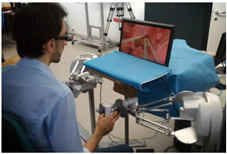
\includegraphics{intro1.png}
    \caption{Example of human/robot integration}
    \label{fig:intro1}
\end{figure}

In this context the “active constraints” (or “virtual fixtures”), are
defined. They are collaborative control strategies, which can be used
to improve or assist human manipulation tasks \cite{acvf}, with a
motion regulation performed by attaching tools to a robotic arm, which
is primarily controlled by the human user. Throughout operation, the
robot controller monitors the tool motion with respect to predefined
trajectories or restricted regions. The active constraint controller
then attenuates or nullifies any user command, which will cause the
manipulator to digress from the plan or enter the restricted region.

There are many different active constraints strategies depending on
some characteristics, for example Regional or Guidance active
constraints, Attractive or Repulsive, Unilateral or
Bilateral\cite{acvf}; the combination of these characteristic is
chosen depending on the application. 

\begin{figure}[h]
    \centering
    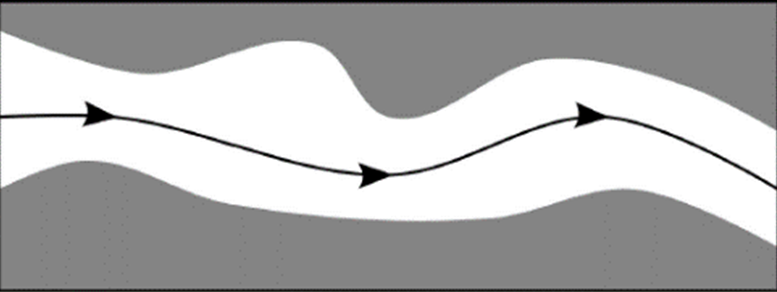
\includegraphics{intro2.png}
    \caption{Example of a guidance active constraint}
    \label{fig:intro2}
\end{figure}
The aim of this work is to create a Guidance active constraint (as in
\textit{Figure \ref{fig:intro2})}, to make a human operator to follow
a predefined trajectory, to protect organs in robot assisted minimally
invasive surgery performed with a Da Vinci machine. This algorithm
implements a viscosity-based dynamic guidance constraint that
continuously redirects the Da Vinci tool’s motion towards the
reference path. A viscosity-based guidance constraints relies on the
concept of viscosity to compute the force that the robot applies on
the tool controlled by the human operator. In particular, the faster
and the more the tool moves away from the desired trajectory, the
bigger the force magnitude will be. The proportionality and continuity
of generated forces make the method not much distracting and
subjectively appealing.

In the following paragraphs it is explained more in detail the
different parts of the project such as the virtual environment
simulation in Unity, the viscosity force computation formulas, and the
actual implementation of the active constraints on the \textit{Da
Vinci Surgical Kit} (DVRK).

\section{Materials and Methods}
Studies and implementations of this specific application of virtual
fixtures have been conducted at first on a simulated environment,
which allowed for a higher flexibility in the development and for a
risk-free testing phase. A virtual operating room has been set up in a
Unity scene, comprehensive of an operating table, two Patient-Side
Manipulators (PSMs) and one Endoscope Camera Manipulator (ECM), as
shown in \textit{Figure \ref{fig:Unity Scene}}. 
\begin{figure}[t]
    \centering
    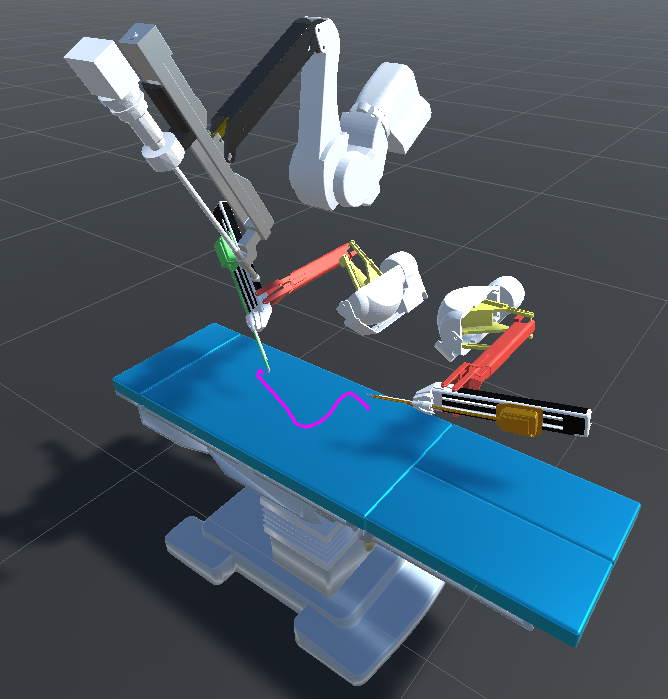
\includegraphics[width=\linewidth]{unityscene.png}
    \caption{Unity Virtual Environment, with two PSMs, one ECM, the path (in magenta) and the operating table.}
    \label{fig:Unity Scene}
\end{figure}
The actuation commands received from the Master Tool Manipulators
(MTMs) at the control station are sent to the Unity environment
through a ROS framework, which will also be the basis for the force
feedback communication once the force vector is computed. Therefore,
the motion from the operator on the MTMs is translated into the motion
of both the end-effector of the PSMs and of the 3D model in the Unity
scene. This approach allows to position a pre-defined path in the
virtual environment, representing the desired trajectory of the
surgical tool: the end-effector position in the real environment is
mimicked by the one in the virtual simulation, which is used to
calculate the force feedback of the active constraint based on the
relative positioning of the end-effector and the path. 

The feedback force computed for the virtual fixture is of viscous
type, as its magnitude depends on the velocity of the end-effector in
space: a more detailed discussion on this kind of active constraint is
given in \cite{equations}. The force magnitude $f$ at each time step
is, in this case, calculated as:
\begin{equation}
    f = \begin{cases}
    b\cdot \norm{\vect{v}} & if \hspace{0.3cm}f<f_{max} \\
    f_{max} & if \hspace{0.3cm} f\geq f_{max}
    \end{cases}
    \label{eq:1}
\end{equation}
$\textbf{v}$ is the velocity vector of the end-effector in space and
$b$ is an anisotropic coefficient obtained as follows:
\begin{equation}
    b = B\cdot\sqrt{\frac{1-\vers{v}\cdot\vers{d}}{2}}
    \label{eq:b}
\end{equation}

Here $\textbf{d}$ is the \textit{deviation}, denoted as the vector
going from the end-effector to the closest point in the path, while
$B$ represents the maximum value of the viscosity coefficient and it
is set by the operator. Equation \ref{eq:b} makes sure that the
coefficient $b$ is maximum when the velocity is opposite to the
deviation (occurring when $\hat{\textbf{v}}\cdot\hat{\textbf{d}}=-1$)
and minimum when the two vectors are aligned
($\hat{\textbf{v}}\cdot\hat{\textbf{d}}=1$). 

The force direction $\hat{\textbf{f}}$ is computed as:
\begin{equation}
    \vers{f} = \begin{cases}
        \vers{d} & if \hspace{0.5cm}\vers{v}\cdot\vers{d}<0\\
        rotate(\vers{v},\theta,\vect{n}) & otherwise
        \label{eq:fvers}
    \end{cases}
\end{equation}
where the $rotate(\cdot)$ function rotates the velocity vector
$\hat{\textbf{v}}$ around the axis denoted by vector
$\hat{\textbf{n}}$ of $\theta$ degrees. Equation \ref{eq:fvers} is
built so that, if the end-effector is moving away from the path (a
condition occurring when the dot product between $\vers{v}$ and
$\vers{d}$ is negative), the force direction is aligned with the
deviation direction, granting therefore independence from the
direction of velocity. Conversely, the vector rotation is applied
solely in the cases where the end-effector approaches the path, and in
this case the angle and axis of rotation are defined as:
\begin{equation}
    \theta = (1+\vers{v}\cdot\vers{d})\cdot\frac{\pi}{2}
\end{equation}
\begin{equation}
    \vect{n} = \vers{v}\times\vers{d}
\end{equation}
Finally, the constraint force $\vect{f}$ is found from the scalar
multiplication
\begin{equation}
    \vect{f} = f\cdot\vers{f}
    \label{eq:force}
\end{equation}
The computation happens in real time during the operation, and a force
vector is hence available at any timestamp and is communicated to the
master controller of the DVRK on a ROS topic.

The ROS framework is essential and covers the whole communication
network between the master controller, the surgical robotic arms and
the virtual environment. For this specific purpose, the relevant ROS
communications are:
\begin{itemize}
    \item The \textit{Joint state} messages published by the PSMs and
    subscribed by the Unity scene, which allow the replication of the
    motion of the real robotic arm by the virtual 3D models
    \item The \textit{Wrench} message published by the Unity virtual
    environment and subscribed by the MTMs, containing the force
    feedback vector
    \item The \textit{gravity compensation} message, which allows to
    account for the effect of gravity when applying the force on the
    MTMs.
\end{itemize}

The force obtained above in Equation \ref{eq:force} is sent, as a ROS
\textit{Twist} object, on the \textit{Wrench} topic which is
subscribed by the master controller.

%%%%%%%%%%%%%%%%%%%%%%%%%%%%%%%%%%%%%%%%%%%%%%%%%%%%%%%%%%%%%%%%%%%%
\textbf{TO DO:} ADD HERE AFTER THE NEXT LAB MEETING
%%%%%%%%%%%%%%%%%%%%%%%%%%%%%%%%%%%%%%%%%%%%%%%%%%%%%%%%%%%%%%%%%%%%
\section{Results}
After the implementation of the methods described above, we collected
data coming from the simulation both for force, velocity and deviation
estimation. As depicted in   \textit{Figure \ref{fig:plots}}, it’s
clear that there exists a trend followed by every single plotted
feature.

\begin{figure*}
    \centering
    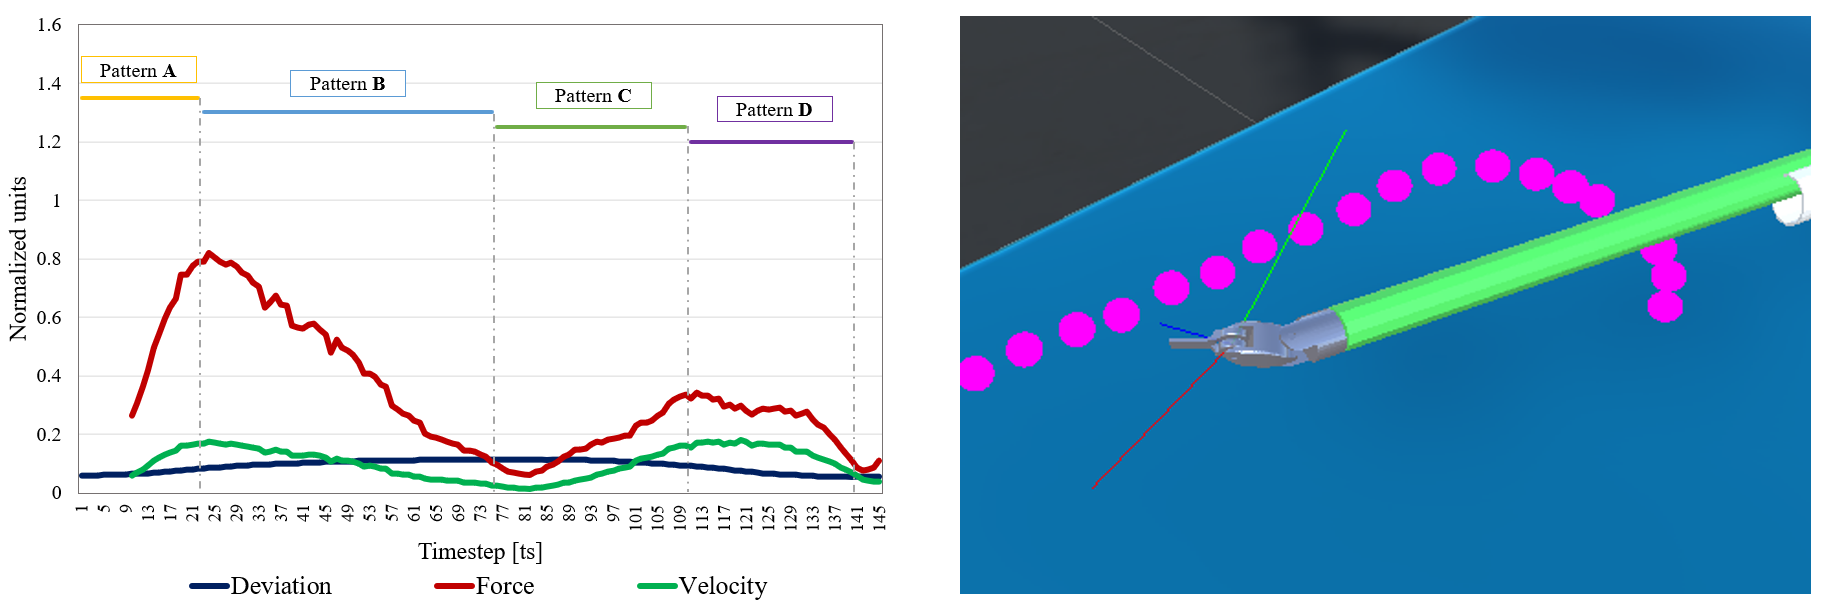
\includegraphics[width=\linewidth]{plotandee.png}
    \caption{\textit{Left:} Magnitude of the force, deviation and
    velocity vectors during movements distancing (Patterns A and B)
    and approaching (Patternss C and D) the predefined path.
    \textit{Right:} Visualization of the three vectors as applied on
    the surgical tool. In magenta, samples from the planned
    trajectory.}
    \label{fig:plots}
\end{figure*}

Please notice that, since the three variables are grouped together, on
the y-axis no unit of measurement is specified, while on the common
x-axis we can find the timestamps, according to the DVRK acquisition
frequency (?????). Furthermore, due to an intrinsic instability in the
virtual models, both for PSMs and ECM, the extracted force, velocity
and normal (not shown, for sake of simplicity) values needed to be
filtered. As we can see from the plots evaluation, the initial raw
data are characterized by an inconvenient noise, which is the origin
of those unreadable spikes and downs. In order to manage the trembling
effects, we applied a moving average, with time period = 18 timestamps
[ts], and overlapped the results to the original raw data, for a
better understanding. This is the reason why only deviation, the blue
line, starts without lagging: force (red) and velocity (green) start
from ts=9, which is the mid-point for the first 18 averaged
timestamps. Furthermore, the magnitude of all three variables clearly
do not hold any information regarding the orientation of such vectors:
for the purpose of the work, the following discussion is considered to
be elucidative enough without decomposing each vector into its three
components, along the cartesian axes, since the direction of each
vector can be deducted from the trend of the other two.

\section{Discussion}

The data acquisition process starts as soon as the MTMs are enabled
for user control [ts=1]. The first increasing trend, around ts=43,
describes the first movement applied to the tool tip: an increase in
deviation means the user was pulling the tool away from the original
path, until ts=103. During this first phase, both force and velocity
have a parabolic behaviour: this is due to the starting and ending
velocity being equal to zero. In fact, force always follows velocity:
while moving far away from the path the computed force tends to
redirect the user in the opposite direction, towards the nearest
point, and its magnitude will increase as long as both velocity and
deviation increase too. Around ts=70 there’s an inversion in the
trend: this is due to the decrease in velocity, even if the tool tip
is still moving away from the path, hence deviation is still
increasing. The descending phase of the deviation [from ts=103 to
ts=157] is as elucidative as the ascending one: as described before,
force still follows velocity, but its increase in magnitude is halved
even if velocity reaches higher values. This behaviour can be
explained again referring to the expressions \ref{eq:1} to
\ref{eq:force}. 

Force computation takes into account both the velocity magnitude and
direction, and it can be seen analysing the force’s parabolic trends
with respect to the deviation derivative, in these four particular
patterns repeated multiple times in \textit{Figure \ref{fig:plots}}.
% \begin{itemize}

\textbf{Pattern A  } Increasing deviation and velocity: the tool tip
is moving away from the path, both the variables have a positive
contribute in the increase of force magnitude. Force and velocity
increase till they both reach local maxima when deviation’s derivative
reaches its peak.

\textbf{Pattern B }  Increasing deviation, decreasing velocity: the
tool tip is still moving away from the path, but is decelerating,
hence deviation is the only positive contribute. Force starts
decreasing and follows velocity’s trend till they both reach local
minima when deviation’s derivative is zero: the tool tip is temporary
still.

\textbf{Pattern C } Decreasing deviation, increasing velocity: the
tool tip has reversed course and started approaching the path at an
increasing velocity, which is the main positive contribute to the
computations. Force starts increasing again, but the decreasing
deviation tends to lower its magnitude, resulting in a parabolic
trend, as for the ascending part, with reduced values. Peaks reached
inside this pattern are the lowest local maxima encountered during
experiments.

\textbf{Pattern D }  Decreasing deviation, decreasing velocity: the
tool tip has almost reached the path, so the user decreases its
velocity. Both deviation and velocity have a negative contribute to
force’s magnitude, which reaches again a local minimum. 


\textbf{Which one of these two?}

--- The local minima, both for velocity and force are reached when the
deviation derivative is zero, hence no difference is noted among the
minima related to approaching and distancing movements

--- Since the local minima, both for velocity and force, are reached
when the deviation derivative is zero, no differences will be noted
between them, as they all fall around zero.


The described pattern can be seen repeated two times in \textit{Figure
\ref{fig:plots}}: please, follow notations inside the plot for a
better understanding.

\section{Conclusions}

\bibliographystyle{plain}
\bibliography{refs}

\end{document}